\documentclass{article}
\usepackage[paperwidth=3.5in, paperheight=4.75in, margin=0.15in]{geometry}
\usepackage[]{graphicx}
\usepackage{float}
\usepackage[T1]{fontenc}

%opening
\title{Device Driver \\I2C Temperature Sensor \\(TI tmp102)}
\author{Ajay Sharma}
\date{2015/02/27}

\begin{document}
\maketitle

\section{CHANGES}
\begin{table}[H]
\centering
 \begin{tabular}{|l|l|l|}
 \hline Version & Description of change & Date \\ 
 \hline 0.1 & First Draft & 2014/08/25\\ 
 \hline
 \end{tabular} 
\caption{Syntax}
\end{table}

\section{USER SPACE ACCESS}
The file \emph{/mnt/mmc/iot\_client.c} is used to allow control of the temperature sensor from the user space. Example of a command to start sending readings to the Carriots server is 
\begin{verbatim}
$ ./iot_client 
\end{verbatim}
The following is read from the driver. The file used is \emph{/sys/bus/i2c/devices/0-0048/temperature\_reg}.
\begin{table}[H]
\centering
 \begin{tabular}{|l|}
 \hline Value \\ 
 \hline 32786 \\
 \hline
 \end{tabular} 
\caption{Sensor Data}
\end{table}

\section{BOARD SUPPORT}
Linux wants to keep board support information in a separate place. In 
\emph{arch/arm/mach-lpc22xx/\\lpc2468\_ea\_board.c} the i2c is setup as below.
The i2c interface operates at 100KHz and P0.28, 27 are used for the I2C functions.
\begin{verbatim}
/*----------------------------------------
*  I2C  
* ----------------------------------------*/
/* I2C board specific data */
struct lpc2xxx_i2c_pdata lpc2xxx_i2c_pdata = 
{ 	
  0,      // fpclk is set in the init 
          // function below
  100000, // freq in Hz 	
  100,    // timeout 
  3,      // retries 
};

static void __init 
lpc2468_ea_init_i2c_pins(void)
{ 	
  lpc2xxx_i2c_pdata.fpclk = lpc_get_fpclk();
#if defined(CONFIG_LPC2XXX_I2C0)
  lpc22xx_set_periph(LPC22XX_PIN_P0_28,1,0);
  // SCL0
  lpc22xx_set_periph(LPC22XX_PIN_P0_27,1,0);
  // SDA0
#endif 
}
\end{verbatim}

\section{DEVICE DRIVER}
An i2c Linux architecture contains bus and client drivers. Bus drivers further contains adapter and algorithm driver. The adapter is the one that is attached directly to the CPU and is sort of acting as an adapter on the system. It can have its own algorithm to support I2C. The algorithm driver is used when the adapter cannot support its own algorithm (Not sure how TBD). The client is connected to the adapter over the I2C bus. Either the adapter or the client can initiate the transfer. They can both act as a slave as well. In the file i2c-lpc2xxx.c, the master I2C hw block in the LPC2468 is registered as an adapter. In tmp102.c, the temperature sensor on the I2C bus which is a slave device is registered as a client.
\subsection{Write Byte}
In a typical I2C write command, there are 3 parts: 
\begin{itemize}
\item Slave Address
\item Command Byte(Register address)
\item Data to be written  
\end{itemize}
The packet information is given below.

\begin{table}[H]
\centering
 \begin{tabular}{|l|l|}
 \hline Packet & Value \\ 
 \hline Slave address & 0x48 \\
 \hline Command byte & TBD \\
 \hline Data & TBD \\
 \hline 
 \end{tabular} 
\caption{Data packet}
\end{table}

% TBD Include the table to read the readings from the sensor
%\begin{figure}[h]
%\label{fig:write_i2c_packets}
%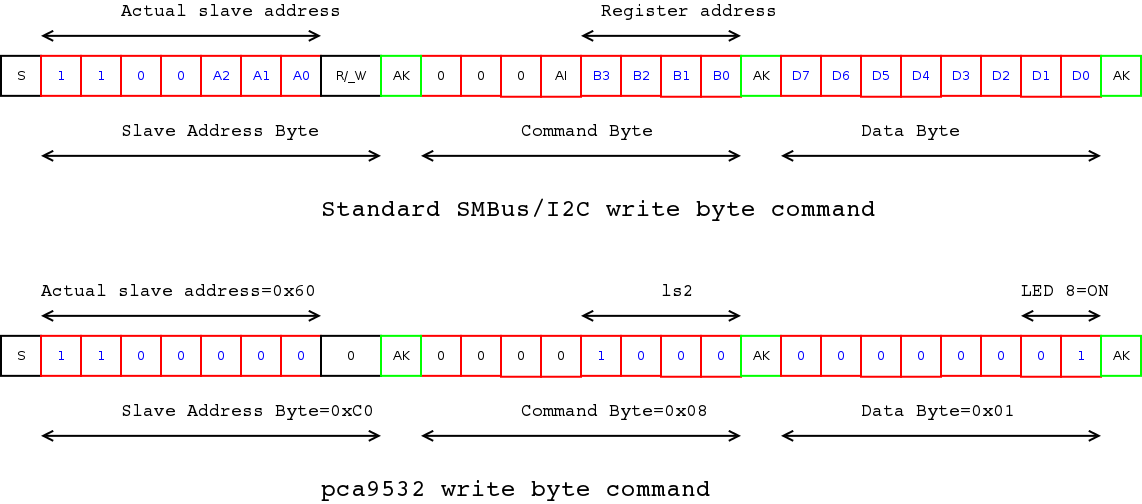
\includegraphics[width=\linewidth]{./write_i2c_packets.png}
%\caption[SMBus/I2C write byte command packets]{}
%\end{figure}

\subsubsection{Command Byte}
The declaration of smbus write function is
\begin{verbatim}
s32 i2c_smbus_read_byte_data
(struct i2c_client *client, u8 command);. 
\end{verbatim}
The i2c\_client is the tmp102, the command is the index set for the command in the device attribute. 
\begin{verbatim}
enum tmp102_cmd { 	...
  TMP102_TEMPERATURE_REG = 0, 	
  TMP102_CONFIG_REG      = 1,
  TMP102_TLOW_REG        = 2,
  TMP102_THIGH_REG       = 3, 
};

#define TMP102_ENTRY_RW(name, cmd_idx) \ 	
  static SENSOR_DEVICE_ATTR(name, \
    S_IRUGO | S_IWUSR, tmp102_show,\
    tmp102_store, cmd_idx) 

TMP102_ENTRY_RO(temperature_reg, TMP102_TEMPERATURE_REG);
TMP102_ENTRY_RW(config_reg, TMP102_CONFIG_REG);
TMP102_ENTRY_RW(tlow_reg, TMP102_TLOW_REG);
TMP102_ENTRY_RW(thigh_reg, TMP102_THIGH_REG);

struct sensor_device_attribute *psa =\
 to_sensor_dev_attr(attr);
....
i2c_smbus_write_byte_data\
  (client, psa->index, val);
\end{verbatim}
When calling the read byte, the psa->index now becomes 0/1/2/3; which turns out to the register address of 0/1/2/3 accordingly. The temperature register is 0. 

\subsubsection{Measurement}
The measurement is little tricky to read. Refer to the datasheet for more information. Here is summary though. 

\begin{table}[H]
\centering
 \begin{tabular}{|l|l|l|l|l|l|l|l|}
 \hline - & - & - & - & T3 & T2 & T1 & T0 \\ 
 \hline 1 & 0 & 0 & 0 & 0 & 0 & 0 & 0 \\
 \hline 
 \end{tabular} 
\caption{Byte 2}
\end{table}

\begin{table}[H]
\centering
 \begin{tabular}{|l|l|l|l|l|l|l|l|}
 \hline T11 & T10 & T9 & T8 & T7 & T6 & T5 & T4 \\ 
 \hline 0 & 0 & 0 & 1 & 0 & 0 & 1 & 0 \\
 \hline 
 \end{tabular} 
\caption{Byte 1}
\end{table}

\begin{table}[H]
\centering
 \begin{tabular}{|l|l|l|l|l|l|}
 \hline Decimal & 32786 \\
 \hline Hex & 0x8012 \\ 
 \hline Binary & 1000\_\textbf{0000\_0001\_0010}\\
               & --------{\scriptsize Byte0----Byte2----Byte1} \\ 
 \hline Reordered 12 bits & 0001\_0010\_0000\\
 \hline Hex & 0x120\\
 \hline Decimal & 288\\
 \hline Final value(x0.0625) & 18 (288 x 0.0625)\\ 
 \hline 
 \end{tabular} 
\caption{Measurement}
\end{table}

\subsubsection{Alarm Registers}
There are two registers that show the high and low reading level upon which the alarm pin is set. The files to read are \emph{/sys/bus/i2c/devices/0-0048/thigh\_reg} and 
\emph{/sys/bus/i2c/devices/0-0048/tlow\_reg}. By default there values are 75,80 respectively. 

\begin{table}[H]
\centering
 \begin{tabular}{|l|l|}
 \hline Register & Value \\ 
 \hline THIGH & 80 \\
 \hline TLOW & 75 \\
 \hline 
 \end{tabular} 
\caption{Alarm registers}
\end{table}

\subsubsection{Configuration Register}
The 4th register shows the current configuration. By default the following values are read.
\begin{table}[H]
\centering
 \begin{tabular}{|l|l|l|l|}
 \hline Symbol & Pos & Val & Meaning\\ 
 \hline SD & 0 & 0 & Shutdown mode\\
 \hline TM & 1 & 0 & Thermostat mode: \\
     &   &   & 0-comparator, 1-Interrupt \\
 \hline \_POL & 2 & 0 & Polarity of Alert pin\\
 \hline F0 & 3 & 0 & Fault Queue\\
 \hline F1 & 4 & 0 & Fault Queue\\
 \hline R0 & 5 & 1 & Convertor Resolution\\
 \hline R1 & 6 & 1 & " - 12 bit \\
 \hline OS & 7 & 0 & One shot conversion\\
 \hline -- & 8 & 0 & NA \\
 \hline -- & 9 & 0 & NA \\
 \hline -- & 10 & 0 & NA \\
 \hline -- & 11 & 0 & NA \\
 \hline EM & 12 & 0 & Extended Mode\\
 \hline AL & 13 & 1 & Alert Bit\\
 \hline CR0 & 14 & 0 & Conversion speed\\
 \hline CR1 & 15 & 1 & " 10 -> 4Hz\\
 \hline 
 \end{tabular} 
\caption{Configuration register}
\end{table}


\subsubsection{Slave Address}
The slave address is 7 bits. Its set constant at 0x48 as the hardware address pins ADD0 is connected to GND. Although the table description may look like \\
1001000, We pad the MSB and put it this way: \\0100\_1000. This make is 0x48. If PIN4 ADD0 pin was connected to VCC, the address would be 0x49\\
(100\_1000). But when we set the register value, we set it with the Read/\_Write flag as well. So now it becomes \\
1001\_000R/W\_, which is now: 0x90(R)/0x91(W\_).
\begin{verbatim}
/* i2c_client_address_data is the struct for 
* holding default client addresses for a 
* driver and for the parameters supplied on 
* the command line  
*/ 
struct i2c_client_address_data { 	
  unsigned short *normal_i2c; 	
  unsigned short *probe; 	
  unsigned short *ignore; 	
  unsigned short **forces; 
}; 

static struct i2c_client_address_data 
addr_data = {\ 
  .normal_i2c = normal_i2c,\
  .probe = probe,\ 
  .ignore = ignore,\
  .forces = forces,\ 
}

/* Addresses to scan */ 
static unsigned short normal_i2c[] = \
{0x48,0x49,0x4A,0x4B,I2C_CLIENT_END}; 
\end{verbatim}
\emph{TBD}
Declared in \emph{i2c.h}, i2c\_client\_address\_data has a static variable definition of addr\_data. Its member variable normal\_i2c is initialized to 0x48.... in the \emph{tmp102.c} file. While writing to the SMBus, the address is used by the i2c driver.

Below is the schematic for TBD on the base oem board. 

%\begin{figure}[h]
%\label{fig:  schematic}
%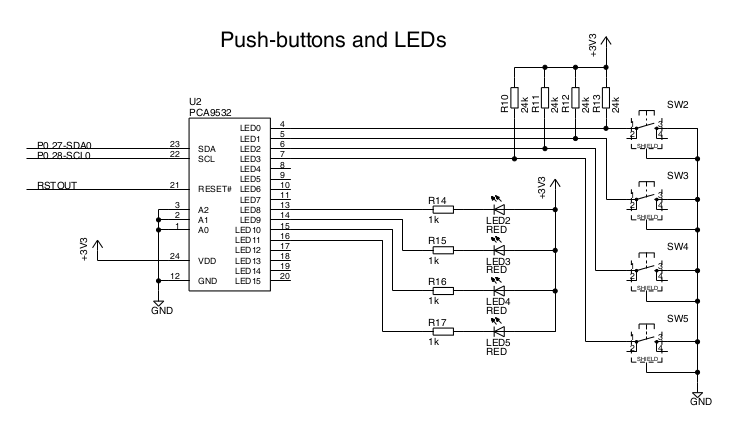
\includegraphics[width=\linewidth]{./pca9532_schematic.png}
%\caption[pca9532 schematic]{}
%\end{figure}

\subsubsection{Call Hierarchy}
Inorder to write to the slave, sysfs file write call the tmp102\_store(). This calls a generic \\ \emph{i2c\_smbus\_write\_byte\_data()} with the client struct, command index(register address) and data value. i2c core file tries to see if the adapter supports smbus\_xfer which should be set to a valid value in the adapter. In lpc24xx its NULL, so an emulated version of smbus is called instead. This emulation fills up data as per SMBus specification and calls i2c\_transfer for the adapter. The lpc2xx adapter driver does fill up the master\_xfer member variable with a valid xfer function which is then called. In the The flow of the call is given below. Similar happens for the read functions.

\begin{verbatim}
974: i2c_smbus_xfer(client->adapter,\
       client->addr,client->flags,\
       I2C_SMBUS_WRITE,command,\
       I2C_SMBUS_BYTE_DATA,&data);
....
1203: res =\
    i2c_smbus_xfer_emulated(adapter,\
       addr,flags,read_write, \
       command,size,data);
...
1157: i2c_transfer(adapter, msg, num);
...
648: ret =\
    adap->algo->master_xfer(adap,msgs,num);
\end{verbatim}

\begin{figure}[h]
\label{fig: i2c driver write process}
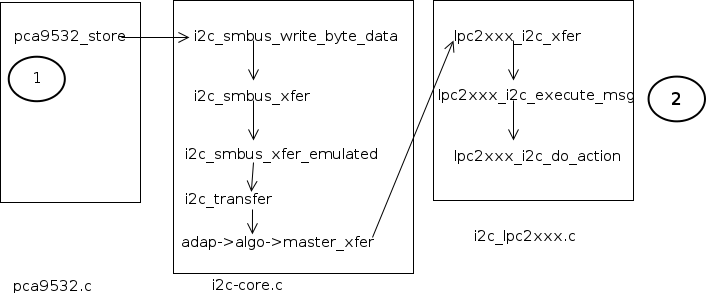
\includegraphics[width=\linewidth]{./write_i2c_flow.png}
\caption[i2c driver write process]{}
\end{figure}



\subsection{Initialization}
When ever a module is loaded to the kernel memory some initialization routines are called. Loading a module is done using either insmod or modprobe. In case of this driver the module init is done using module\_init function. 
\begin{verbatim}
module_init(tmp102_init);
\end{verbatim}
Here the function tmp102\_init is passed as a parameter and is defined with the type \_\_init type. This means its loaded before the main function is called. 
\begin{verbatim}
static int __init tmp102_init(void)
\end{verbatim}
\emph{tmp102\_init} calls \emph{i2c\_add\_driver()} to add a static driver data structure to the i2c core. Details of i2c driver structure is below.
\begin{verbatim}
/*This is the driver that will be inserted */ 

static struct i2c_driver tmp102_driver = { 
  .driver = { 
    .name = "tmp102", 
  }, 
  .attach_adapter = tmp102_attach_adapter, 
  .detach_client = tmp102_detach_client, 
};
\end{verbatim}
Prototpye for the i2c\_driver is below:


Driver writer is required to fill in the name for the driver. Also \emph{attach\_adapter} and \emph{detach\_client} are functions passed. <TBD> why is attach\_adapter and detach\_client? why not adapter, adapter or client client? 

% TBD
%\begin{figure}[h]
%\label{fig: i2c client init}
%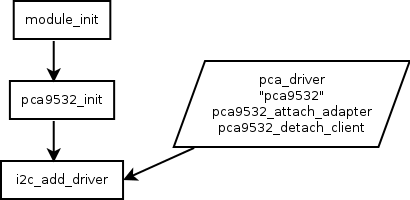
\includegraphics[width=\linewidth]{./i2c_client_init.png}
%\caption[i2c client init]{}
%\end{figure}


\subsubsection{Detection}
In creating a device driver for the tmp102 its required to provide functions that get triggered when the adapter is attached. When the adapter is initialized the tmp102\_attach\_adapter is called. The prototype of attach\_adapter is given below. This function then calls i2c\_probe passing the tmp102\_detect function. 

\begin{verbatim}
static int tmp102_attach_adapter
(struct i2c_adapter *adapter);
\end{verbatim}

\emph{i2c\_probe} function requires the following arguments: 
\begin{verbatim}
int i2c_probe
(struct i2c_adapter *adapter, \
 struct i2c_client_address_data *address_data, 
 int (*found_proc) \
 (struct i2c_adapter *, int, int));
\end{verbatim}

It needs an adapter structure, the client address structure and a procedure to call when a client is attached? The found procedure prototype matches our detect function below. Obviously tmp102\_detect is then called. 

\begin{verbatim}
static int tmp102_detect
(struct i2c_adapter *adapter, int address, \
int kind);
\end{verbatim}

138: In the detection phase, the client checks its adapter's functionality to see if its supports SMBus byte data transfers. The check functionality function is defined in linux-2.6.x./include/linux/i2c.h as an inline function. The adapter(i2c-lpc2xxx.c) initializes a i2c\_algorithm structure with a functionality of I2C and SMBus emulation and a method that is returning it. The check returns positive since the SMBus emulation does mean that the SMBus write bytes are supported. Functionality masks are \#defined in the i2c.h file as well. 

143: Now space is allocated for the client structure using kzalloc. kzalloc allocates memory which is set to zero. GFP\_KERNEL is passed as a flag to the memory allocation inorder to block waiting for the memory allocation. Kernel does its best to try and allocate the memory and the process may sleep waiting for the memory allocation. This is by default the best choice. Prototype of i2c\_client structure is given below. i2c\_set\_clientdata sets the client in the struct device. This structure is defined in linux/device.h. It probably holds the highest level of device data? <TBD: Double check>. Address, driver structure and flags(0) is set for the client. 

22: Inorder to set the address, i2c\_probe function searches struct i2c\_client\_address\_data for the normal\_i2c[] address. i2c\_client\_address\_data is a static struct with a member variable normal\_i2c in the i2c.h header file and so it is required to define normal\_i2c[] in the tmp102.c file. 

166: Finally the i2c\_attach\_client() is called to attach this new client to the device core. 

170: sysfs hook ups are created with the default attribute. 

\subsubsection{Detachment}
Inorder to detach the client, it is removed by calling sysfs\_remove\_group, i2c\_detach\_client and freeing the kernel memory for the client by kfree. 



\subsection{Structure reference}
The various structures used here are described in linux-2.6.x/include/linux/i2c.h file.
Prototype of \\ \emph{i2c\_client\_address\_data} is below:
\begin{verbatim}
/* i2c_client_address_data is the struct for 
* holding default client addresses for a 
* driver and for the parameters supplied on 
* the command line  
*/ 
struct i2c_client_address_data{ 	
  unsigned short *normal_i2c; 	
  ... 
}; 

/*  
 * i2c_adapter is the structure used to 
 * identify a physical i2c bus along with 
 * the access algorithms necessary to access 
 * it.  
 */ 
struct i2c_adapter { 	
  struct module *owner; 	
  .... 	
  /* the algorithm to access the bus */
  const struct i2c_algorithm *algo; 
  ....	
  ....
};


/* 
* A driver is capable of handling one 
* or more physical devices present on 
* I2C adapters. This information is used 
* to inform the driver of adapter 
* events. 
* 
* The driver.owner field should be set to
* the module owner of this driver. 
* The driver.name field should be set to 
* the name of this driver. 
*/
struct i2c_driver { 
  int id; 
  unsigned int class;
  
  /* Notifies the driver that a new bus 
  * has appeared. This routine can be used 
  * by the driver to test if the bus 
  * meets its conditions & seek for the 
  * presence of the chip(s) it supports. 
  * If found, it registers the client(s) 
  * that are on the bus to the i2c admin. 
  * via i2c_attach_client. 
  */ 
  int (*attach_adapter)(struct i2c_adapter *); 
  int (*detach_adapter)(struct i2c_adapter *);

  /* tells the driver that a client is about
   to be deleted & gives it the chance to 
   remove its private data. Also, if the 
   client struct has been dynamically 
   allocated by the driver in the function 
   above, it must be freed here. */ 
  int (*detach_client)(struct i2c_client *);
  ...
  ...
  struct device_driver driver; 
  ...
};

/* 
* i2c_client identifies a single device 
* (i.e. chip) that is connected to an 
* i2c bus. The behaviour is defined by 
* the routines of the driver. This 
* function is mainly used for lookup & 
* other admin. functions. 
*/ 
struct i2c_client { 
/* div., see below */ 
unsigned int flags;   
/* chip address - NOTE: 7bit   */ 
 * addresses are stored in the */ 
 * _LOWER_ 7 bits 
 */ 
unsigned short addr;  
/* the adapter we sit on */ 
struct i2c_adapter *adapter; 
/* and our access routines */ 
struct i2c_driver *driver;   
...
...
char name[I2C_NAME_SIZE]; 
...
};
\end{verbatim}

\end{document}
